
\documentclass[a4paper,11pt]{article}
\usepackage[a4paper, margin=8em]{geometry}

% usa i pacchetti per la scrittura in italiano
\usepackage[french,italian]{babel}
\usepackage[T1]{fontenc}
\usepackage[utf8]{inputenc}
\frenchspacing 

% usa i pacchetti per la formattazione matematica
\usepackage{amsmath, amssymb, amsthm, amsfonts}

% usa altri pacchetti
\usepackage{gensymb}
\usepackage{hyperref}
\usepackage{standalone}

% imposta il titolo
\title{Appunti Comunicazioni Numeriche}
\author{Luca Seggiani}
\date{2026}

% imposta lo stile
% usa helvetica
\usepackage[scaled]{helvet}
% usa palatino
\usepackage{palatino}
% usa un font monospazio guardabile
\usepackage{lmodern}

\renewcommand{\rmdefault}{ppl}
\renewcommand{\sfdefault}{phv}
\renewcommand{\ttdefault}{lmtt}

% disponi il titolo
\makeatletter
\renewcommand{\maketitle} {
	\begin{center} 
		\begin{minipage}[t]{.8\textwidth}
			\textsf{\huge\bfseries \@title} 
		\end{minipage}%
		\begin{minipage}[t]{.2\textwidth}
			\raggedleft \vspace{-1.65em}
			\textsf{\small \@author} \vfill
			\textsf{\small \@date}
		\end{minipage}
		\par
	\end{center}

	\thispagestyle{empty}
	\pagestyle{fancy}
}
\makeatother

% disponi teoremi
\usepackage{tcolorbox}
\newtcolorbox[auto counter, number within=section]{theorem}[2][]{%
	colback=blue!10, 
	colframe=blue!40!black, 
	sharp corners=northwest,
	fonttitle=\sffamily\bfseries, 
	title=~\thetcbcounter: #2, 
	#1
}

% disponi definizioni
\newtcolorbox[auto counter, number within=section]{definition}[2][]{%
	colback=red!10,
	colframe=red!40!black,
	sharp corners=northwest,
	fonttitle=\sffamily\bfseries,
	title=~\thetcbcounter: #2,
	#1
}

% U.D.M
\newcommand{\amp}{\ensuremath{\mathrm{A}}}
\newcommand{\volt}{\ensuremath{\mathrm{V}}}
\newcommand{\meter}{\ensuremath{\mathrm{m}}}
\newcommand{\second}{\ensuremath{\mathrm{s}}}
\newcommand{\farad}{\ensuremath{\mathrm{F}}}
\newcommand{\henry}{\ensuremath{\mathrm{H}}}
\newcommand{\siemens}{\ensuremath{\mathrm{S}}}

% circuiti
\usepackage{circuitikz}
\usetikzlibrary{babel}

% disegni
\usepackage{pgfplots}
\pgfplotsset{width=10cm,compat=1.9}

% disponi codice
\usepackage{listings}
\usepackage[table]{xcolor}

\lstdefinestyle{codestyle}{
		backgroundcolor=\color{black!5}, 
		commentstyle=\color{codegreen},
		keywordstyle=\bfseries\color{magenta},
		numberstyle=\sffamily\tiny\color{black!60},
		stringstyle=\color{green!50!black},
		basicstyle=\ttfamily\footnotesize,
		breakatwhitespace=false,         
		breaklines=true,                 
		captionpos=b,                    
		keepspaces=true,                 
		numbers=left,                    
		numbersep=5pt,                  
		showspaces=false,                
		showstringspaces=false,
		showtabs=false,                  
		tabsize=2
}

\lstdefinestyle{shellstyle}{
		backgroundcolor=\color{black!5}, 
		basicstyle=\ttfamily\footnotesize\color{black}, 
		commentstyle=\color{black}, 
		keywordstyle=\color{black},
		numberstyle=\color{black!5},
		stringstyle=\color{black}, 
		showspaces=false,
		showstringspaces=false, 
		showtabs=false, 
		tabsize=2, 
		numbers=none, 
		breaklines=true
}

\lstdefinelanguage{javascript}{
	keywords={typeof, new, true, false, catch, function, return, null, catch, switch, var, if, in, while, do, else, case, break},
	keywordstyle=\color{blue}\bfseries,
	ndkeywords={class, export, boolean, throw, implements, import, this},
	ndkeywordstyle=\color{darkgray}\bfseries,
	identifierstyle=\color{black},
	sensitive=false,
	comment=[l]{//},
	morecomment=[s]{/*}{*/},
	commentstyle=\color{purple}\ttfamily,
	stringstyle=\color{red}\ttfamily,
	morestring=[b]',
	morestring=[b]"
}

% disponi sezioni
\usepackage{titlesec}

\titleformat{\section}
	{\sffamily\Large\bfseries} 
	{\thesection}{1em}{} 
\titleformat{\subsection}
	{\sffamily\large\bfseries}   
	{\thesubsection}{1em}{} 
\titleformat{\subsubsection}
	{\sffamily\normalsize\bfseries} 
	{\thesubsubsection}{1em}{}

% disponi alberi
\usepackage{forest}

\forestset{
	rectstyle/.style={
		for tree={rectangle,draw,font=\large\sffamily}
	},
	roundstyle/.style={
		for tree={circle,draw,font=\large}
	}
}

% disponi algoritmi
\usepackage{algorithm}
\usepackage{algorithmic}
\makeatletter
\renewcommand{\ALG@name}{Algoritmo}
\makeatother

% disponi numeri di pagina
\usepackage{fancyhdr}
\fancyhf{} 
\fancyfoot[L]{\sffamily{\thepage}}

\makeatletter
\fancyhead[L]{\raisebox{1ex}[0pt][0pt]{\sffamily{\@title \ \@date}}} 
\fancyhead[R]{\raisebox{1ex}[0pt][0pt]{\sffamily{\@author}}}
\makeatother

\begin{document}
% sezione (data)
\section{Lezione del 03-03-26}

% stili pagina
\thispagestyle{empty}
\pagestyle{fancy}

% testo
\subsection{Introduzione}
Il corso mira a dare un introduzione ai \textbf{segnali}, analogici e digitali.

In particolare, gli argomenti trattati sono:
\begin{itemize}
	\item Analisi di \textit{Fourier} di segnali analogici;
	\item Sistemi lineari e filtri;
	\item Teorema di campionamento di \textit{Nyquist-Shannon};
	\item Teoria dei codici;
	\item Sistemi di comunicazione \textit{base-band} e \textit{pass-band}
\end{itemize}

Inoltre, ci saranno alcuni elementi di:
\begin{itemize}
	\item Elementi di probabilità;
	\item Variabili aleatorie;
	\item Processi stocastici.
\end{itemize}

\subsubsection{Note storiche}
Per avere un po' di introduzione storica, possiamo dire che la disciplina che studia i segnali nasce nel 1948 con la \textit{teoria dell'informazione} di \textit{Claude Shannon} (e la successiva \textit{teoria dei codici} di \textit{Golay} e \textit{Hamming}, del 1949).

Una delle più grandi applicazioni di questa tecnologia è \textit{Internet}, derivato dall'\textit{ARPANET} del 1990 (di cui vediamo oggi innumerevoli applicazioni, fra cui il \textit{World Wide Web} del 1990).

Un'altro campo di vasta applicazione della teoria dei segnali è quello delle comunicazioni \textit{wireless}, che nasce dalla teoria di \textit{Maxwell} e da esperimenti come quelli di \textit{Bell} e \textit{Marconi} di inizio '900.
Oggi la tecnologia delle reti mobili si è evoluta per \textit{generazioni} (1G, 2G, ...). Notiamo come evoluzioni più importanti il 2G \textit{GSM} e il 4G \textit{LTE} (\textit{Long Term Evolution}), che riesce ad avere vaste aree di copertura usando un approccio in \textit{divisione di frequenza} (\textit{FDMA}).

\subsubsection{Teoria dell'informazione}
La \textbf{teoria dell'informazione}, come abbiamo detto, viene formalizzata da Shanno nel 1948. 
Ciò che si voleva capire era la \textbf{capacità} di bit al secondo che si potevano trasferire per un canale di comunicazione digitale (basato su bit 1/0) ad una certa frequenza (in $\mathrm{Hz}$).
Nel dettaglio, si va a ricavare la seguente formula (teorema di \textit{Shannon-Hartley}):
$$
\text{Capacity} = \text{Bandwidth} \log_2 \left( 1 + \frac{\text{Signal}}{\text{Noise}} \right) \, \mathrm{bit}/\mathrm{s}/\mathrm{Hz}
$$

La \textbf{banda} è la frequenza a cui siamo capaci di trasmettere informazione sul mezzo, mentre chiamiamo \textbf{throughput} la frequenza di trasmissione di informazione effettiva che otteniamo.
Possiamo dire che la capacità non è altro che il throughput che otteniamo sulla data banda:
$$
\text{Capacity} = \frac{\text{Throughput}}{\text{Bandwidth}}
$$

Notiamo subito come è importante il \textit{rapporto segnale-rumore} (\textbf{SNR}) per valutare la cosiddetta capacità \textit{raggiungibile} dai sistemi di comunicazione. Disegnamo la zona raggiungibile nel seguente grafico, dove il SNR si evolve in maniera esponenziale sull'asse delle ascisse:
\begin{center}
	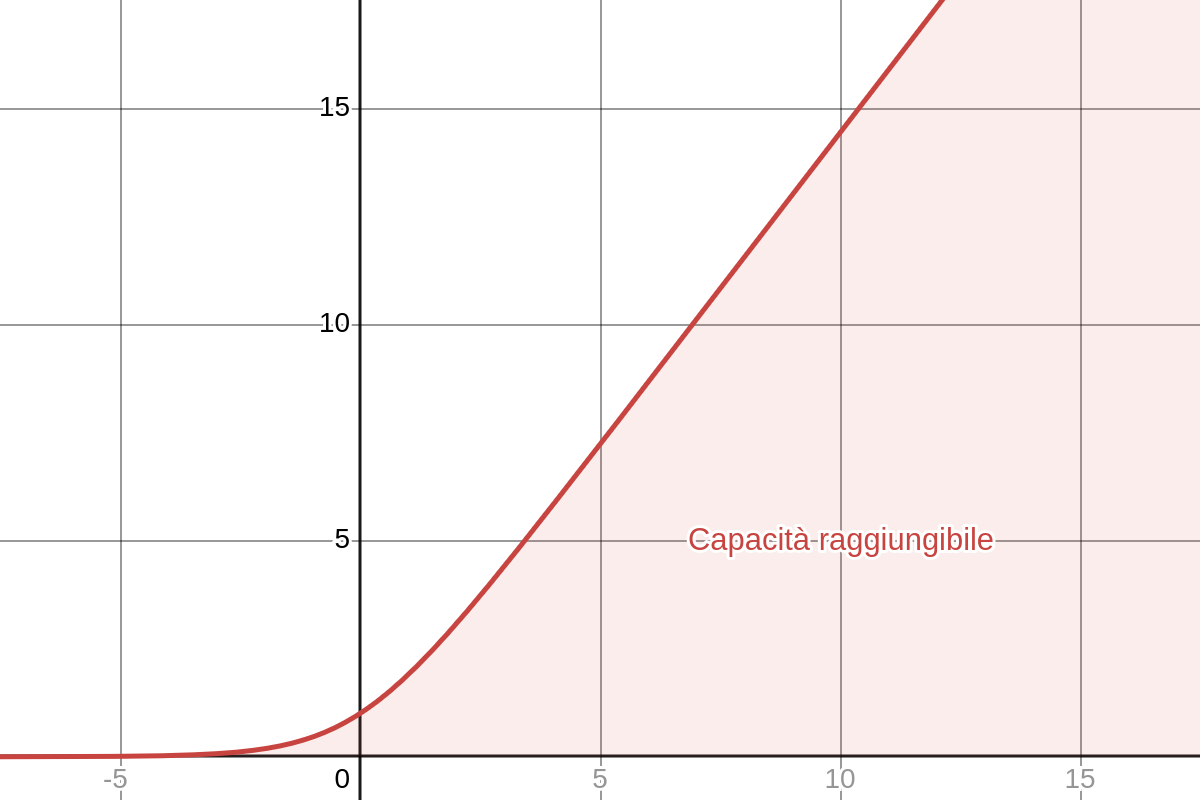
\includegraphics[scale=0.3]{../figures/shannon_hartley.png}
\end{center}

Notiamo che la capacità definita da Shannon è sì la massima raggiungibile su un mezzo, ma la sua teoria non ci dà alcuna informazione riguardo a come effettivamente raggiungerla.

\subsection{Elementi di un sistema di comunicazione}
Interroghiamoci quindi su cos'è nel dettaglio un \textbf{sistema di comunicazione}.

\begin{center}
	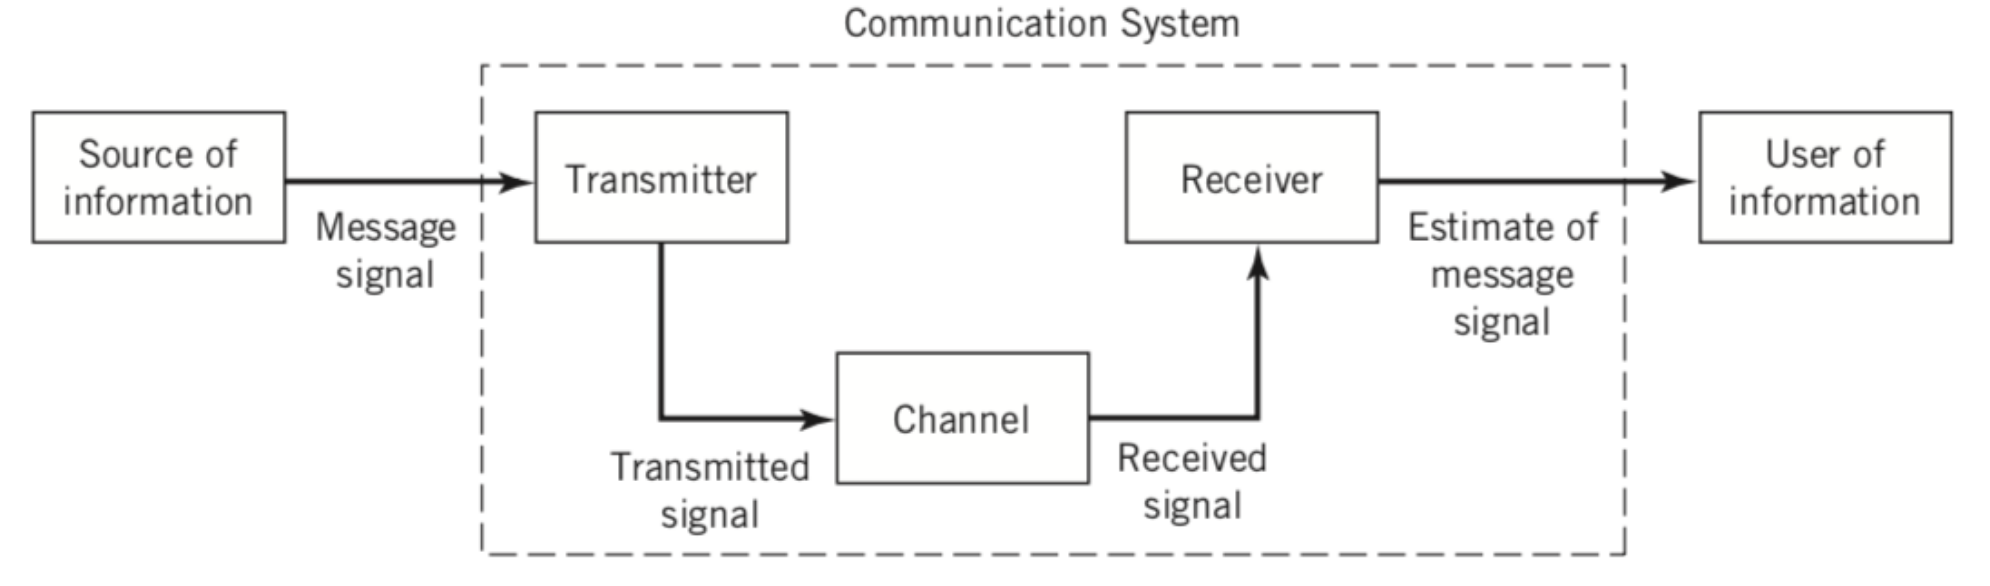
\includegraphics[scale=0.2]{../figures/sys_simp.png}
\end{center}

Di base, questo è un sistema composto da:
\begin{itemize}
	\item Un \textbf{trasmettitore} che trasmette l'informazione proveniente da una \textit{sorgente} sotto forma di \textit{segnale};
	\item Un \textbf{mezzo} attraverso il quale si propaga il segnale;
	\item Un \textbf{ricevitore} che riceve il segnale e lo riporta in informazione per consegnarla all'\textit{utente} dell'informazione.
\end{itemize}

In verità, possiamo vedere il sistema più nel dettaglio:
\begin{center}
	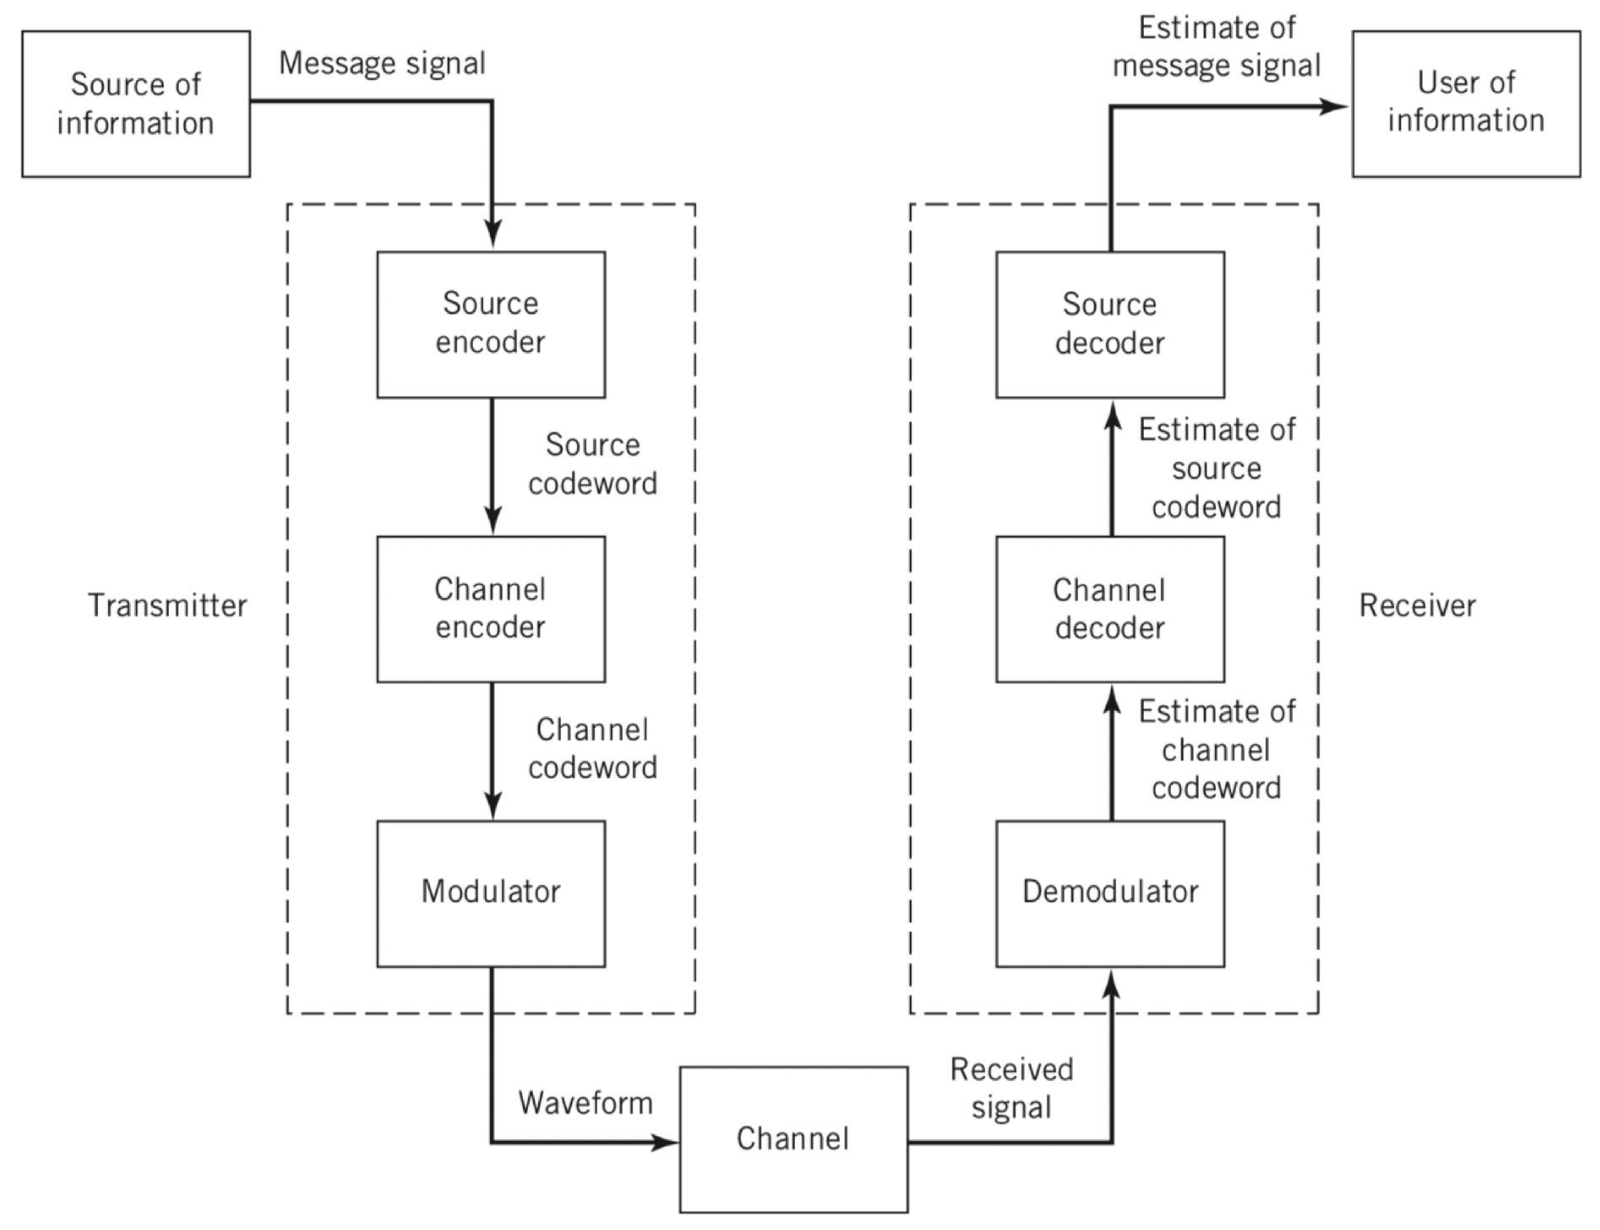
\includegraphics[scale=0.25]{../figures/sys_comp.png}
\end{center}
\begin{itemize}
	\item Vediamo i componenti da cui è composto il \textbf{trasmettitore}:
		\begin{itemize}
			\item \textbf{Source encoder}: sfrutta la \textit{ridondanza} del messaggio con l'obiettivo di ridurne le dimensioni, senza comunque perdere troppa dell'informazione originale da non renderne possibile la decodifica in seguito.

				L'esempio tipico che possiamo fare è quello degli algoritmi di \textit{compressione} in uso nei calcolatori, ad esempio prima di caricare file di grandi dimensioni in rete;
			\item \textbf{Channel encoder}: prende il messaggio ricevuto dal \textit{source encoder} e lo prepara alla trasmissione sul canale. in questo caso notiamo che fa la cosa opposta: introduce della nuova ridondanza in modo da compensare gli errori che verranno commessi sul canale di propagazione.

				L'introduzione di ridondanza nei messaggi per la correzione degli errori si basa su un'intuizione semplice: anche gli esseri umani potrebbero, quando non capiscono un messaggio, chiedere di \textit{ripeterlo}: è appunto questa ripetizione apparentemente ridondante che permette di recuperare un errore e proseguire con la comunicazione.
				
				Chiaramente, la ridondanza presenta un \textit{tradeoff}: l'energia spesa a trasmettere informazione ridondante poteva essere usata per trasmettere nuova informazione, e va quindi tenuta ad un livello minimo.

				Durante il corso studieremo i codici \textbf{a blocco}, che sono codici \textit{lineari} studiabili attraverso gli strumenti dell'algebra lineare; 
			\item \textbf{Modulator}: quello che esce dal modulatore non è più il segnale digitale preso dal channel encoder, ma una \textit{forma d'onda} adatta a essere trasmessa sul mezzo.
		\end{itemize}

	\item Vediamo quindi l dettaglio dei componenti del \textbf{ricevitore}, che saranno perlopiù parallelli a quelli del trasmettitore:
		\begin{itemize}
			\item \textbf{Demodulator}: si occuperà di trasformare forme d'onda sul mezzo in bit, che sperabilmente saranno i bit emessi dal \textit{channel encoder} del trasmettitore;
			\item \textbf{Channel decoder}: si occuperà di sfruttare l'operazione ridondante inserita dal \textit{channel encoder} per ricostruire il messaggio originale generato dal \textit{source encoder};
			\item \textbf{Source decoder}: si occuperà di invertire il processo effettuato dal \textit{source encoder}, in maniera da ricostruire il messaggio originale.
		\end{itemize}
\end{itemize}

\subsubsection{Modello OSI}
Il modello \textbf{OSI} (\textit{Open System Interconnect}) fornisce uno standard per l'organizzazione su \textit{livelli} di un sistema di comunicazione. Possiamo dire che il livello che abbiamo visto finora è il cosiddetto livello \textit{fisico}.

\begin{center}
	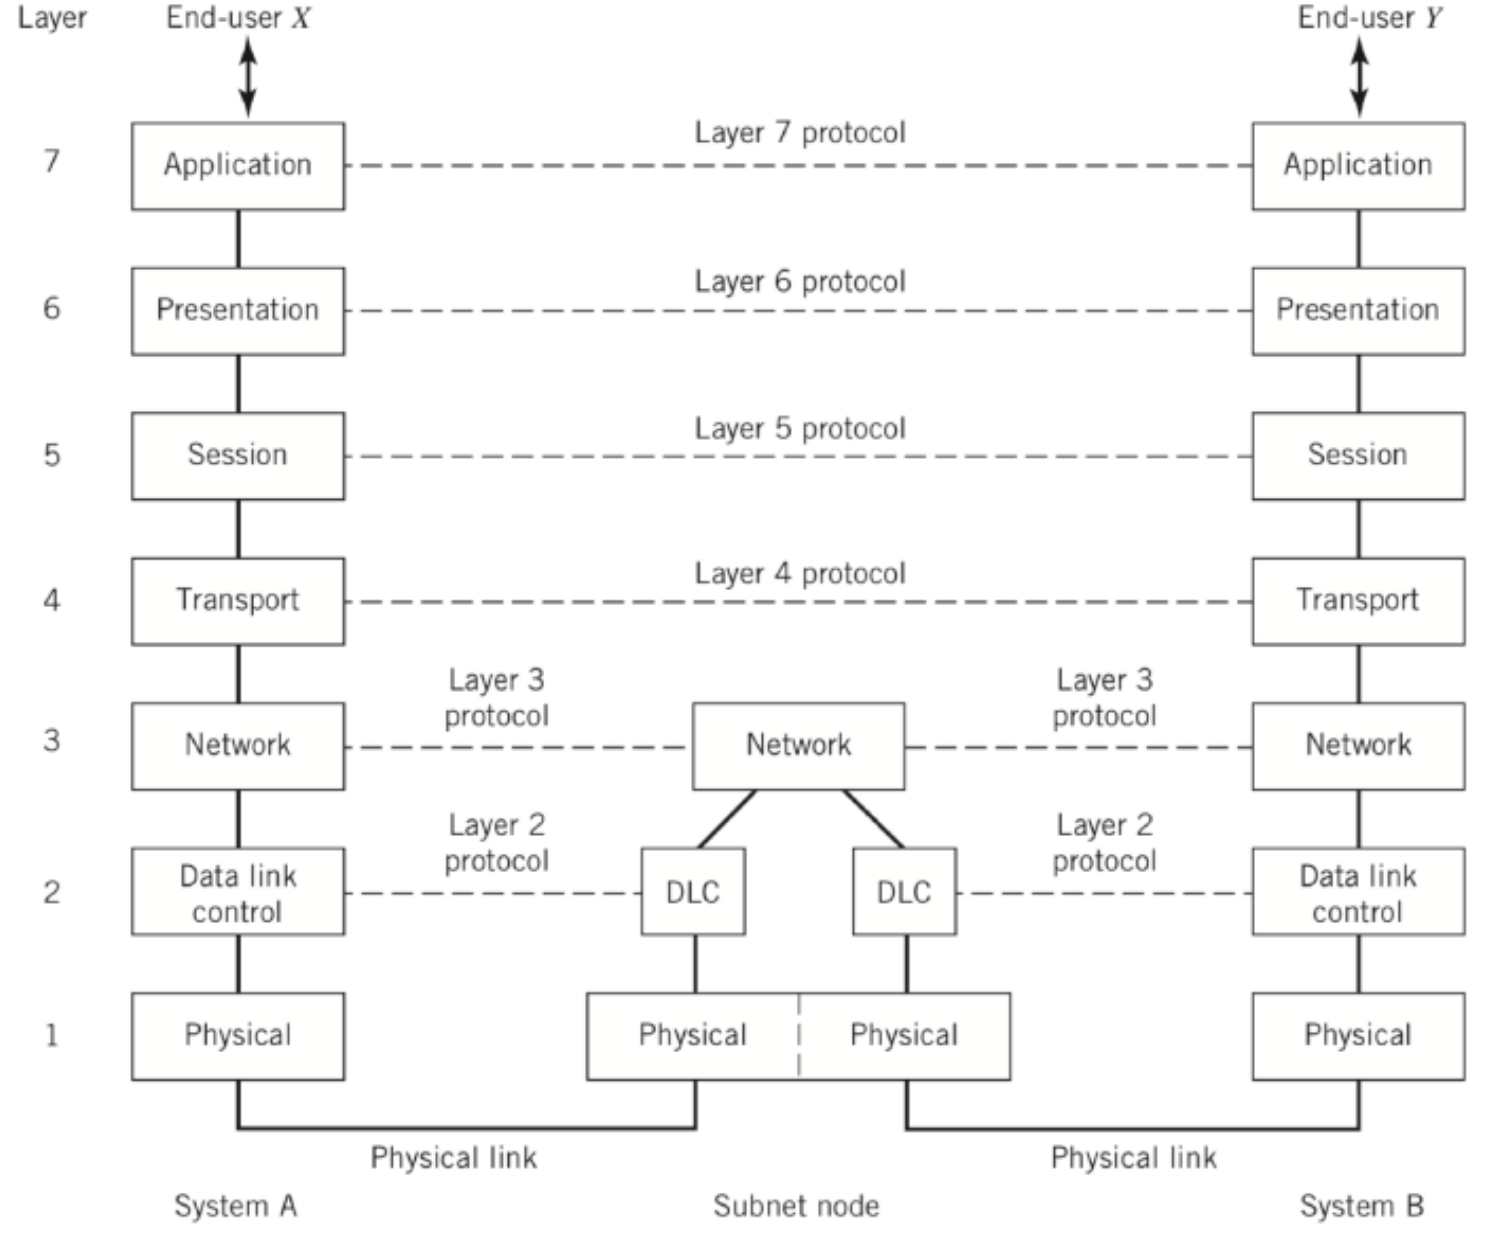
\includegraphics[scale=0.275]{../figures/osi.png}
\end{center}

Assieme a questo, il modello OSI prevede 7 livelli:
\begin{itemize}
	\item Livello \textbf{application}, quello a cui operano le applicazioni vere e proprie che interessano agli utenti;
	\item Livello \textbf{presentation}, un livello introdotto per trasformare i dati in ingresso in un formato comprensibile alle macchine degli utenti (gestendo particolarità come byte ordering, ecc...);
	\item Livello \textbf{session}, un livello introdotto per gestire le \textit{sessioni} degli utenti;
	\item Livello \textbf{transport}, a cui si assicura la ridondanza ad alto livello dell'informazione e quindi la corretta trasmissione di dati anche attraverso diversi \textit{hop} (\textit{"salti"});
	\item Livello \textbf{network}, a cui si permette l'\textit{interconnessione} di reti attraverso un formato comune;
	\item Livello \textbf{datalink}, costruito sul livello \textit{physical}, pensato per prendersi a carico il trasferimento di dati da questo alle macchine utente, e introdurre in alcuni casi un suo livello di ridondanza;
	\item Livello \textbf{physical}, quello che abbiamo visto finora, riguardante il \textit{mezzo fisico} vero e proprio;
\end{itemize}

Del modello OSI notiamo che è modulare e quindi semplice da sviluppare ed estendere.
Abbiamo che la maggior parte delle cose che accadono nelle comunicazioni digitali avvengono ai livelli \textbf{physical}, \textbf{datalink} e \textbf{network}.

\subsubsection{Struttura delle reti}
Le reti sono formate da una serie di \textbf{nodi} interconnessi fra di loro. Il compito dei nodi è quello di instradare dati attraverso la rete, ed ogni nodo può avere una o più stazioni agganciate ad esso.

Esistono 2 tipi principali di rete:
\begin{itemize}
	\item Rete a \textbf{commutazione di circuito}, dove le interconnessioni fra i nodi che collegano 2 stazioni in comunicazione vengono allocate completamente a quella comunicazione: altri nodi non possono usare le interconnessioni finché la comunicazione non è finita.

		Un esempio tipico è quello del \textbf{POTS} (\textit{Plain Old Telephone Service}), cioè la comune rete telefonica;
	\item Rete a \textbf{commutazione di pacchetto}, dove sulla rete non circolano segnali ma \textit{pacchetti}, cioè elementi finiti di informazione che vengono ricavati dal segnale vero e proprio e possono quindi viaggiare in maniera \textit{interlacciata} sul mezzo. Usato un approccio a comunicazione di pacchetto si può avere un uso condiviso da parte di più stazioni della stessa interconnessione.

		L'esempio più celebre di rete a commutazione di pacchetto è la comune rete \textit{Internet}.
\end{itemize}

\subsubsection{Modalità di comunicazione}
Su una rete si possono avere diverse \textbf{modalità} di comunicazione

\begin{itemize}
	\item \textbf{Broadcasting}, dove un singolo nodo trasmette a più ricevitori;
	\item \textbf{Point-to-point}, dove la comunicazione avvene su un singolo link fra un trasmettitore e un ricevitore;
	\item \textbf{Point-to-multipoint}, dove la comunicazione avviene su un link fra un trasmettitore e più ricevitori.
\end{itemize}

\subsubsection{Accesso multiplo}
Diversi mezzi sono condivisi da più trasmettitori, cioè hanno bisogno di un protocollo \textbf{MAC} (\textit{Medium Access Control}) per governare l'accesso al mezzo e fornire:
\begin{itemize}
	\item Divisione del mezzo fra i trasmettitori;
	\item Sicurezza da \textit{collisioni} fra le comunicazioni dei trasmettitori.
\end{itemize}

Esistono diversi approcci per effettuare l'accesso condiviso. In particolare notiamo:
\begin{itemize}
	\item \textbf{TDMA} (\textit{Time Division Multiple Access}): si divide l'uso del mezzo in più \textit{slot} temporali, allocati ognuno ad un diverso trasemttitore.

		Ad esempio, viene usata nei sistemi cellulari di seconda generazione (2G);
	\item \textbf{FDMA} (\textit{Frequency Division Multiple Access}): si divide lo \textit{spettro} del mezzo in più \textit{bande} di frequenza, allocata ognuna ad un diverso trasemttitore.

		Ad esempio, viene usata nei sistemi cellulari di quarta generazione (4G) assieme al TDMA.

\begin{center}
	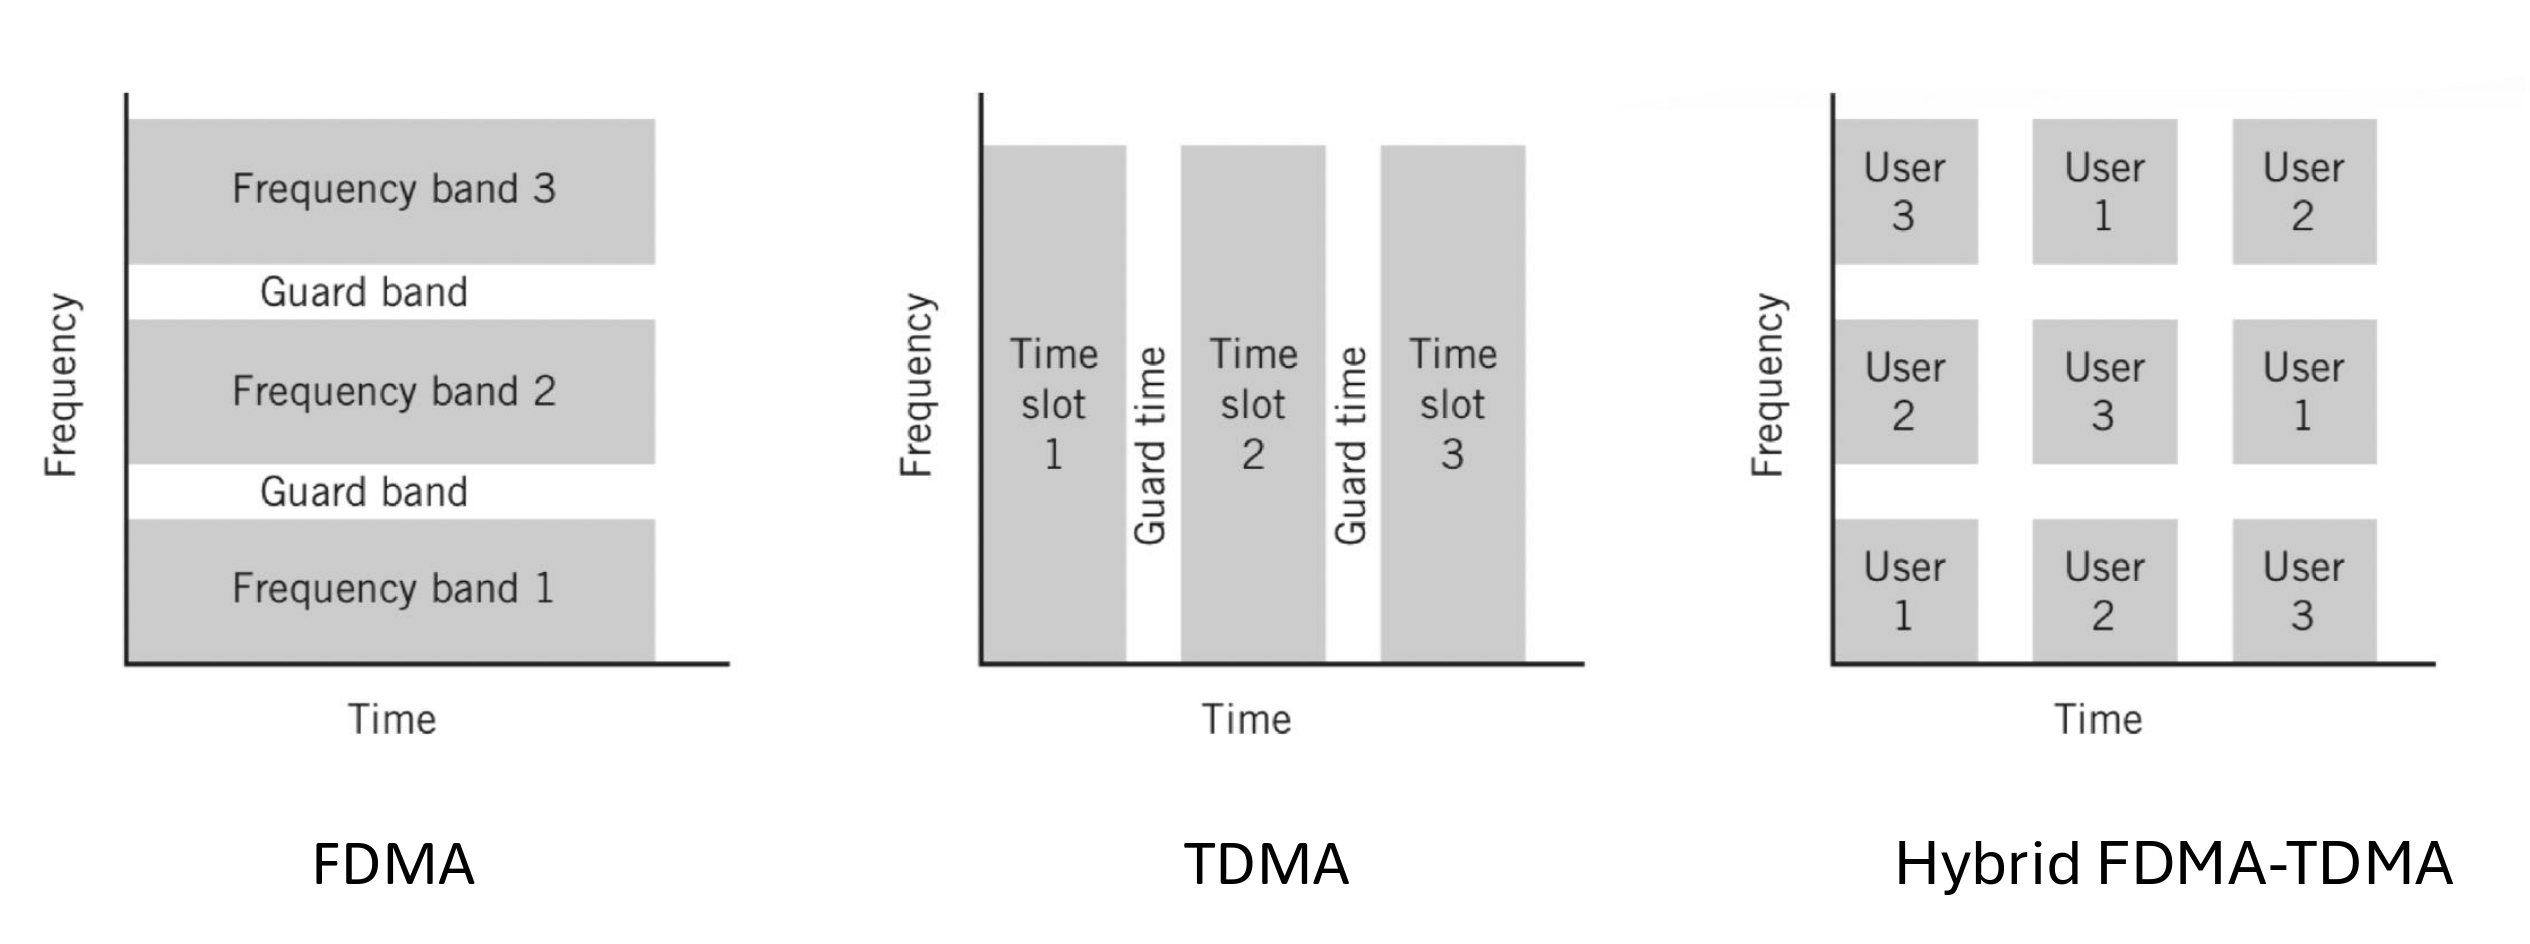
\includegraphics[scale=0.15]{../figures/4g_part.png}
\end{center}

		In particolare, possiamo dire che il 4G \textit{LTE} sfrutta un apporccio \textit{ibrido} FDMA-TDMA, dove si divide il mezzo sia in slot temporali che bande di frequenza, ottenendo quindi una sorta di \textit{matrice} di slot disponibili per la trasmissione. Questi slot possono quindi essere allocati dalle \textit{base station} ai dispositivi cellulari in maniera dinamica, per permettere la comunicazione sulla rete. 
	\item \textbf{CDMA} (\textit{Code Division Multiple Access}): si associa ad ogni dispositivo trasmettitore un \textit{codice}. Questi codici verranno progettati in maniera da non interferire se più dispositivi comunicano contemporaneamente: sempre per questo motivo il partizionamento dei codici si comporta in maniera simile al partizionamento degli slot temporali o delle bande di frequenza.

		Ad esempio, è stata introdotta in ambito militare e ha poi trovato applicazione nei sistemi cellulari di terza generazione (3G);
	\item \textbf{SDMA} (\textit{Space Division Multiple Access}): in questo caso si usa la separazione spaziale degli utenti per effettuare la condivisione del mezzo. In questo caso si possono allocare più slot del mezzo prevedendo più antenne per dispositivo. 

		Ad esempio, viene applicata nei sistemi cellulari di quinta generazione (5G), nell'ambito delle \textit{onde millimetriche}.
\end{itemize}

Notiamo che ognuna delle modalità di condivisione del mezzo fornisce una qualche "unità" minima (slot temporale, banda, codice) che può essere allocata ad un dispositivo. Per aumentare la capacità di trasmissione di un singolo dispositivo, nulla ci vieta di allocare più unità di trasmissione ad un singolo dispositivo.

\subsubsection{Spettro delle radiofrequenze}
Lo spettro delle radiofrequenze usate per la comunicazione \textit{wireless} va dai 3 Hz ai 300 GHz (vediamo che oltre i 300 GHz l'\textit{attuenazione} del segnale è troppo alta da dare risultati utili).

Abbiamo che questo spettro è usato in maniera condivisa da diversi sistemi, fra cui ad esempio la trasmissione televisiva, le reti mobili, le reti Wi-Fi IEEE 802.11x e Bluetooth, ecc...
Sono quindi definiti degli enti che allocano e regolamentano lo spazio delle frequenze radio in modo da fornire uno slot abbastanza grande a tutte le applicazioni.

Vediamo una tabella riassuntiva delle bande di radiofrequenze usate e le applicazioni per cui vengono usate:
\begin{table}[h!]
\center
\rowcolors{2}{white}{black!10}
\begin{tabular}{ c | c | c }
\bfseries Nome & \bfseries Banda (Frequenze) & \bfseries Uso \\
\hline
ELF & 3–30 Hz & Comunicazioni sottomarine \\
SLF & 30–300 Hz & Comunicazioni sottomarine \\
ULF & 300 Hz–3 kHz & Comunicazioni speciali, geofisica \\
VLF & 3–30 kHz & Navigazione, comunicazioni militari \\
LF  & 30–300 kHz & Radiofari, navigazione \\
MF  & 300 kHz–3 MHz & Radio AM \\
HF  & 3–30 MHz & Onde corte, comunicazioni a lunga distanza \\
VHF & 30–300 MHz & FM, TV, aeronautica \\
UHF & 300 MHz–3 GHz & TV digitale, cellulari, Wi-Fi \\
SHF & 3–30 GHz & Radar, satelliti, microonde \\
EHF & 30–300 GHz & Comunicazioni ad onde millimetrali, ricerca \\
\end{tabular}
\end{table}

Notiamo che la frequenza allocata è più o meno inversamente proporzionale all'area di copertura del sistema: per sistemi a corto raggio come il Wi-Fi IEEE 802.11x si può sfruttare la banda \textit{ISM} a 2.4 GHz o della banda a 5 GHz, mentre per sistemi come la radio FM si usano le bande \textit{VHF} dagli 87.5 MHz ai 108.0 MHz, ad esempio.

\subsection{Richiami di analisi}
Abbiamo bisogno di fare alcuni richiami di analisi in modo da avviarci verso l'analisi di \textit{Fourier}.

\subsubsection{Numeri complessi}
Un numero \textbf{complesso} $\in \mathbb{C}$ è rappresentato da parte reale e immaginaria, come:
$$
z = a + ib
$$
dove $i$ è l'\textit{unità immaginaria}, con la proprietà:
$$
i^2 = -1
$$

Definiamo i classici operatori \textit{parte reale} e \textit{parte immaginaria}:
$$
a = \mathrm{Re}\{z\}, \quad b = \mathrm{Im}\{z\}
$$

\par\smallskip

\noindent
\textbf{\textsf{Coniugato}}

\noindent
Di un numero complesso si può calcolare il \textbf{coniugato} come:
$$
z^* = a - ib
$$

Valgono le seguenti proprietà, di facile dimostrazione:
$$
a = \mathrm{Re}\{z\} = \frac{z + z^*}{2}, \quad b = \mathrm{Im}\{z\} = \frac{z - z^*}{2}
$$

\par\smallskip

\noindent
\textbf{\textsf{Forma polare}}

\noindent
Assieme alla rappresentazione $z = a + ib$ appena vista, detta rappresentazione \textbf{cartesiana}, esiste la cosiddetta rappresentazione \textbf{polare} di un numero complesso:
$$
z = c e^{i \theta}, \quad
\begin{cases}
	c = \sqrt{a^2 + b^2} \\
	\theta = \mathrm{atan2}(b, a)
\end{cases}, \quad
\begin{cases}
	a = c \cos(\theta) \\
	b = c \sin(\theta)
\end{cases}
$$

dove l'esponenziale $e^{i \theta}$ ruota un numero nello spazio complesso dell'angolo $\theta$ attorno all'origine (questo si ricava dalla scomposizione nella serie di Taylor della funzione esponenziale con argomento complesso, la cui dimostrazione si può trovare nei testi di analisi).

\par\smallskip

\noindent
\textbf{\textsf{Operazioni sui complessi}}

\noindent
Come sempre, ricordiamo che:
\begin{itemize}
	\item Le \textbf{somme} complesse sono semplici in rappresentazione cartesiana:
		$$
			z_1 + z_2 = (a_1 + a_2) + i(b_1 + b_2) =
		$$
	\item I \textbf{prodotti} complessi sono semplici in rappresentazione polare:
		$$
			z_1 \cdot z_2 = (a_1 a_2 - b_1 b_2) + (a_1 b_2 + a_2 b_1) = c_1 c_2 e^{i(\theta_1 + \theta_2)}
		$$

		Per quanto riguarda le \textit{divisioni}, ricordiamo l'identità utile:
		$$
			\frac{z_1}{z_2} = \frac{z_1}{z_2} \frac{z_2^*}{z_2^*} = \frac{z_1 z_2^*}{|z_2|^2}
		$$
		da cui:
		$$
		\frac{z_1}{z_2} = \frac{(a_1 a_2 + b_1 b_2) + (a_2 b_1 - a_1 b_2)}{a_2^2 + b_2^2} = \frac{c_1}{c_2} e^{i(\theta_1 - \theta_2)}
		$$
\end{itemize}

\subsubsection{Seno e coseno}
Definiamo le funzioni \textbf{seno} e \textbf{coseno} di un angolo $\theta$ rispettivamente come la posizione alle ascisse e alle ordinate di un punto con angolo $\theta$ in coordinate polari sulla circonferenza unitaria.
Ricordiamo la celebre identità:
$$
\sin^2(\theta) + \cos^2(\theta) = 1
$$
data dal teorema di \textit{Pitagora}.


\par\smallskip

\noindent
\textbf{\textsf{Formule di Eulero}}

\noindent
Esiste una corrispondenza fra seno, coseno e numeri complessi rappresentata dalle identità:
$$
\cos(\theta) = \frac{e^{i \theta} + e^{-i \theta}}{2}, \quad \cos(\theta) = \frac{e^{i \theta} - e^{-i \theta}}{2i}
$$
dette formule di \textit{Eulero}, che stanno alla base della conversione fra forme cartesiane e polari dei numeri complessi viste prima in 1.3.2 (sempre prima avevamo accennato alla derivazione formale di queste formule). 

\end{document}
